\documentclass[12pt, a4paper]{article}
\usepackage[spanish]{babel}
\usepackage[utf8]{inputenc}
\usepackage{graphicx}
\usepackage{geometry}
\usepackage{fancyhdr}
\usepackage{float}
\usepackage{titling}
\usepackage{hyperref}
\usepackage{url}




% Márgenes
\geometry{a4paper, margin=2.5cm}

% Encabezado y pie de página
\pagestyle{fancy}
\fancyhf{}
\rhead{
\includegraphics[height=1.2cm]{images/logo-usm.png}}
\lhead{Grupo 19\\Visualización de Datos}
\rfoot{Página \thepage}

% Configuración del logo en portada
\pretitle{
  \begin{center}
  \vspace{1cm}
  
\includegraphics[width=0.5\textwidth]{images/logo-usm.png}\\
  \vspace{1.5cm}
  \LARGE
}
\posttitle{\end{center}}

% Título del informe
\title{Percepciones y Uso de la Inteligencia Artificial}
\author{Felipe Campaña, Javier Gómez, Matias Elgueta}
\date{\today\\[2cm]}

\begin{document}
\maketitle

% ---------------------------------------------------------------------------------
\section*{Criterios de Selección}
\begin{itemize}
    \item Criterio 1: Frecuencia de uso de IA
    \item Criterio 2: Principales usos de IA	
    \item Criterio 3: Confianza en IA
    \item Criterio 4: Frecuencia vs Confianza
    \item Criterio 5: Preocupación laboral
    \item Criterio 6: Uso principal vs Preocupación laboral	
\end{itemize}



% ---------------------------------------------------------------------------------
\section*{Análisis por Integrante}

% ===================== FELIPE CAMPAÑA =====================
\subsection*{Integrante 1: Felipe Campaña}

\subsubsection*{Criterios Seleccionados}
\begin{itemize}
    \item Frecuencia de uso de IA.
    \item Principales usos de IA.
\end{itemize}

\subsubsection*{Justificación: Frecuencia de uso de IA.}
Este indicador representa la regularidad con la que las personas usan herramientas con inteligencia artificial en su vida diaria, desde un uso esporádico hasta un uso intensivo.

\begin{itemize}
    \item Permite medir el nivel de exposición tecnológica y familiaridad de los usuarios con la IA.
    \item Da cuenta del grado de integración de estas herramientas en rutinas personales o académicas.
    \item Es útil para interpretar otras variables como confianza, percepción o utilidad de la IA.
\end{itemize}

\subsubsection*{Justificación: Principales usos de IA.}
Este indicador muestra los fines más comunes para los cuales se utiliza la inteligencia artificial, como estudiar, crear arte, buscar ideas o programar.

\begin{itemize}
    \item Ayuda a identificar el enfoque funcional que los usuarios dan a la IA en su vida cotidiana.
    \item Refleja cómo las personas aprovechan estas herramientas en contextos académicos, creativos o recreativos.
    \item Es clave para entender el tipo de valor que los usuarios perciben en estas tecnologías.
\end{itemize}


\subsubsection*{Gráfico 1: Frecuencia de uso de IA.}
\begin{figure}[H]
    \centering
    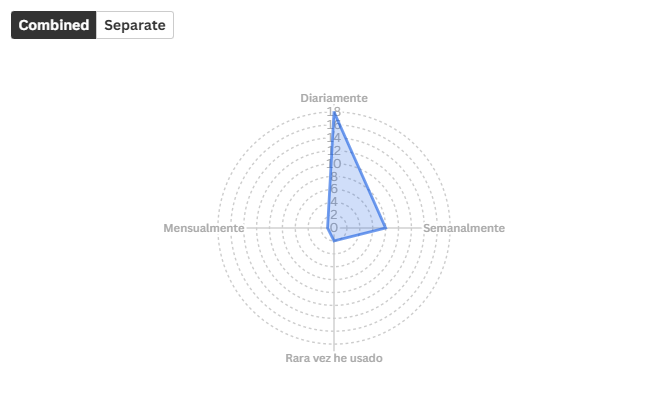
\includegraphics[width=0.85\textwidth]{Graficos/Radar_frec_ia_FC.png}
    \caption[1]{Fuente: Elaboración propia con datos}
\end{figure}

\textbf{Conclusión:}
\begin{itemize}
    \item La mayoría de los encuestados utiliza la IA principalmente para estudiar (65\% del total).
    \item Los usos relacionados con programación (17\%) y búsqueda de ideas (10\%) ocupan el segundo y tercer lugar.
    \item El uso recreativo o de entretención representa una minoría (7\%), lo que indica un enfoque más académico o productivo.
    \item El gráfico evidencia que la IA es percibida como una herramienta funcional más que como una distracción.
\end{itemize}

\subsubsection*{Gráfico 2: Principales usos de IA.}
\begin{figure}[H]
    \centering
    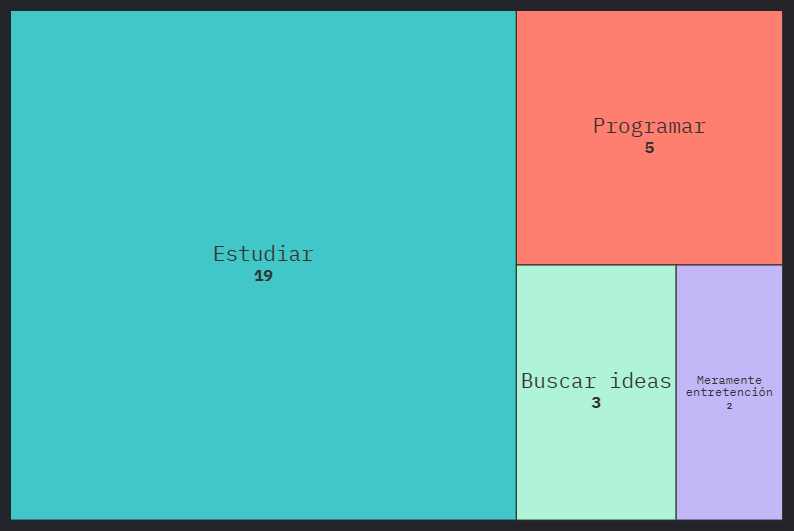
\includegraphics[width=0.85\textwidth]{Graficos/Treemap_Uso_IA_FC.png}
    \caption[2]{Fuente: Elaboración propia con datos}
\end{figure}

\textbf{Conclusión:}
\begin{itemize}
    \item El uso diario de IA destaca significativamente, representando la categoría con mayor frecuencia entre los encuestados.
    \item El uso semanal también es relevante, aunque menor en comparación con el uso diario.
    \item El gráfico sugiere una integración intensiva de la IA en las rutinas diarias de los participantes.
    \item Esto puede reflejar tanto una alta dependencia como una adaptación natural al uso frecuente de estas tecnologías.
\end{itemize}


% ===================== JAVIER GÓMEZ =====================
\newpage
\subsection*{Integrante 2: Javier Gómez}

\subsubsection*{Criterios Seleccionados}
\begin{itemize}
    \item 
    \item 
\end{itemize}

\subsubsection*{Justificación: }
Permite .

\begin{itemize}
    \item 
    \item 
\end{itemize}

\subsubsection*{Justificación: }
Revela .
\begin{itemize}
    \item 
\end{itemize}

\subsubsection*{Gráfico 3: }
\begin{figure}[H]
    \centering
    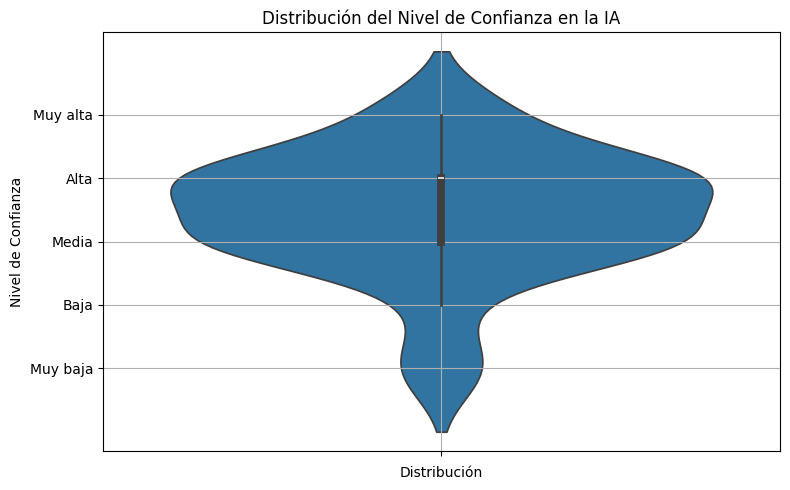
\includegraphics[width=0.85\textwidth]{Graficos/beeswarn.png}
    \caption[3]{Fuente: Elaboración propia con datos}
\end{figure}

\newpage
\textbf{Conclusión:}  
\begin{itemize}
    \item Como se puede ver en el gráfico, países como Brasil, Nigeria, Filipinas y Chile lideran el ranking en cuanto a uso diario de redes sociales, con promedios superiores a las 3 horas diarias. En general, los países de América Latina y África muestran un uso bastante elevado, lo que refleja lo presentes que están estas plataformas en la vida cotidiana de sus habitantes.
    \item Por otro lado, en países como Japón, Alemania o Bélgica, el tiempo promedio dedicado a redes sociales es mucho menor. Esto puede estar relacionado con diferencias culturales o incluso con estilos de vida donde quizás se priorizan otras formas de comunicación.
    \item El lector podría encontrar interesante realizar un estudio frente a la relación entre cantidad de horas frente a, por ejemplo, rendimiento académico $\bullet{}\bigcirc{}\bullet{}$
\end{itemize}

\subsubsection*{Gráfico 4: }
\begin{figure}[H]
    \centering
    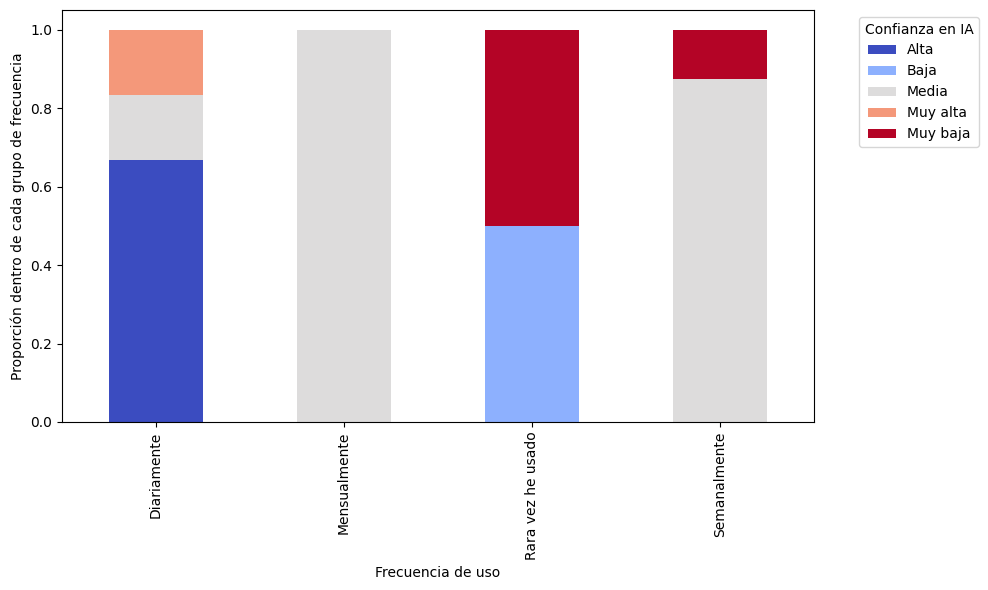
\includegraphics[width=0.85\textwidth]{Graficos/spin plot.png}
    \caption[4]{Fuente: Elaboración propia con datos}

\end{figure}


\textbf{Conclusión:}  
\begin{itemize}
    \item Este gráfico muestra la evolución del número de clientes por empresa en los últimos años. Lo más destacable es el aumento significativo de las suscripciones a servicios móviles durante la pandemia \(2020-2021\).
    Durante esos años, varias empresas, como WOM y ENTEL, experimentaron un fuerte crecimiento, probablemente impulsado por la necesidad de mantenerse conectados desde casa, ya sea por trabajo, estudios o simplemente para mantenerse en contacto con los demás.
    \item También es notable cómo algunas empresas han mantenido una base de clientes más estable a lo largo del tiempo, mientras que otras, como VTR Móvil, tienen una participación mucho menor. En 2024, ENTEL se destacó como la empresa con más clientes, superando los 215.000, lo que podría indicar una estrategia comercial sólida o una percepción positiva de su servicio.

\end{itemize}


% ===================== MATÍAS ELGUETA =====================
\subsection*{Integrante 3: Matías Elgueta}

\subsubsection*{Criterios Seleccionados}
\begin{itemize}
    \item Criterio 1: 
    \item Criterio 2: 
\end{itemize}

\subsubsection*{Justificación:}
Nos permite observar cómo es percibida la recolección y utilización de nuestros datos personales por personas de distintas edades, lo que puede ser útil para:

\begin{itemize}
    \item Diseñar campañas de concientización específicas por grupo etario, enfocándose en los públicos que muestran menor preocupación o menor conocimiento sobre el uso de sus datos.
    \item Adaptar políticas de privacidad y términos de uso en plataformas digitales, considerando el nivel de confianza que cada grupo etario tiene respecto al tratamiento de sus datos personales.
\end{itemize}

\subsubsection*{Justificación: Penetracion 5G}
Nos permite visualizar la evolución para la penetración de la red 5G entre 2015 y 2025 en distintos países, lo que facilita la comparación del ritmo de adopción tecnológica a nivel internacional y revela posibles brechas digitales, lo que puede ser útil para:
\begin{itemize}
    \item Tomar decisiones de inversión en infraestructura tecnológica, identificando países con mayor crecimiento 5G, lo cual puede orientar estrategias de empresas del sector de telecomunicaciones.
    \item Diseñar políticas públicas o marcos regulatorios que impulsen una adopción más equitativa de tecnologías avanzadas, especialmente en países con baja penetración, fomentando así la inclusión digital.
\end{itemize}

\subsubsection*{Gráfico 4: Preocupación ante el uso no autorizado de datos personales por rango etario.}
\begin{figure}[H]
    \centering
    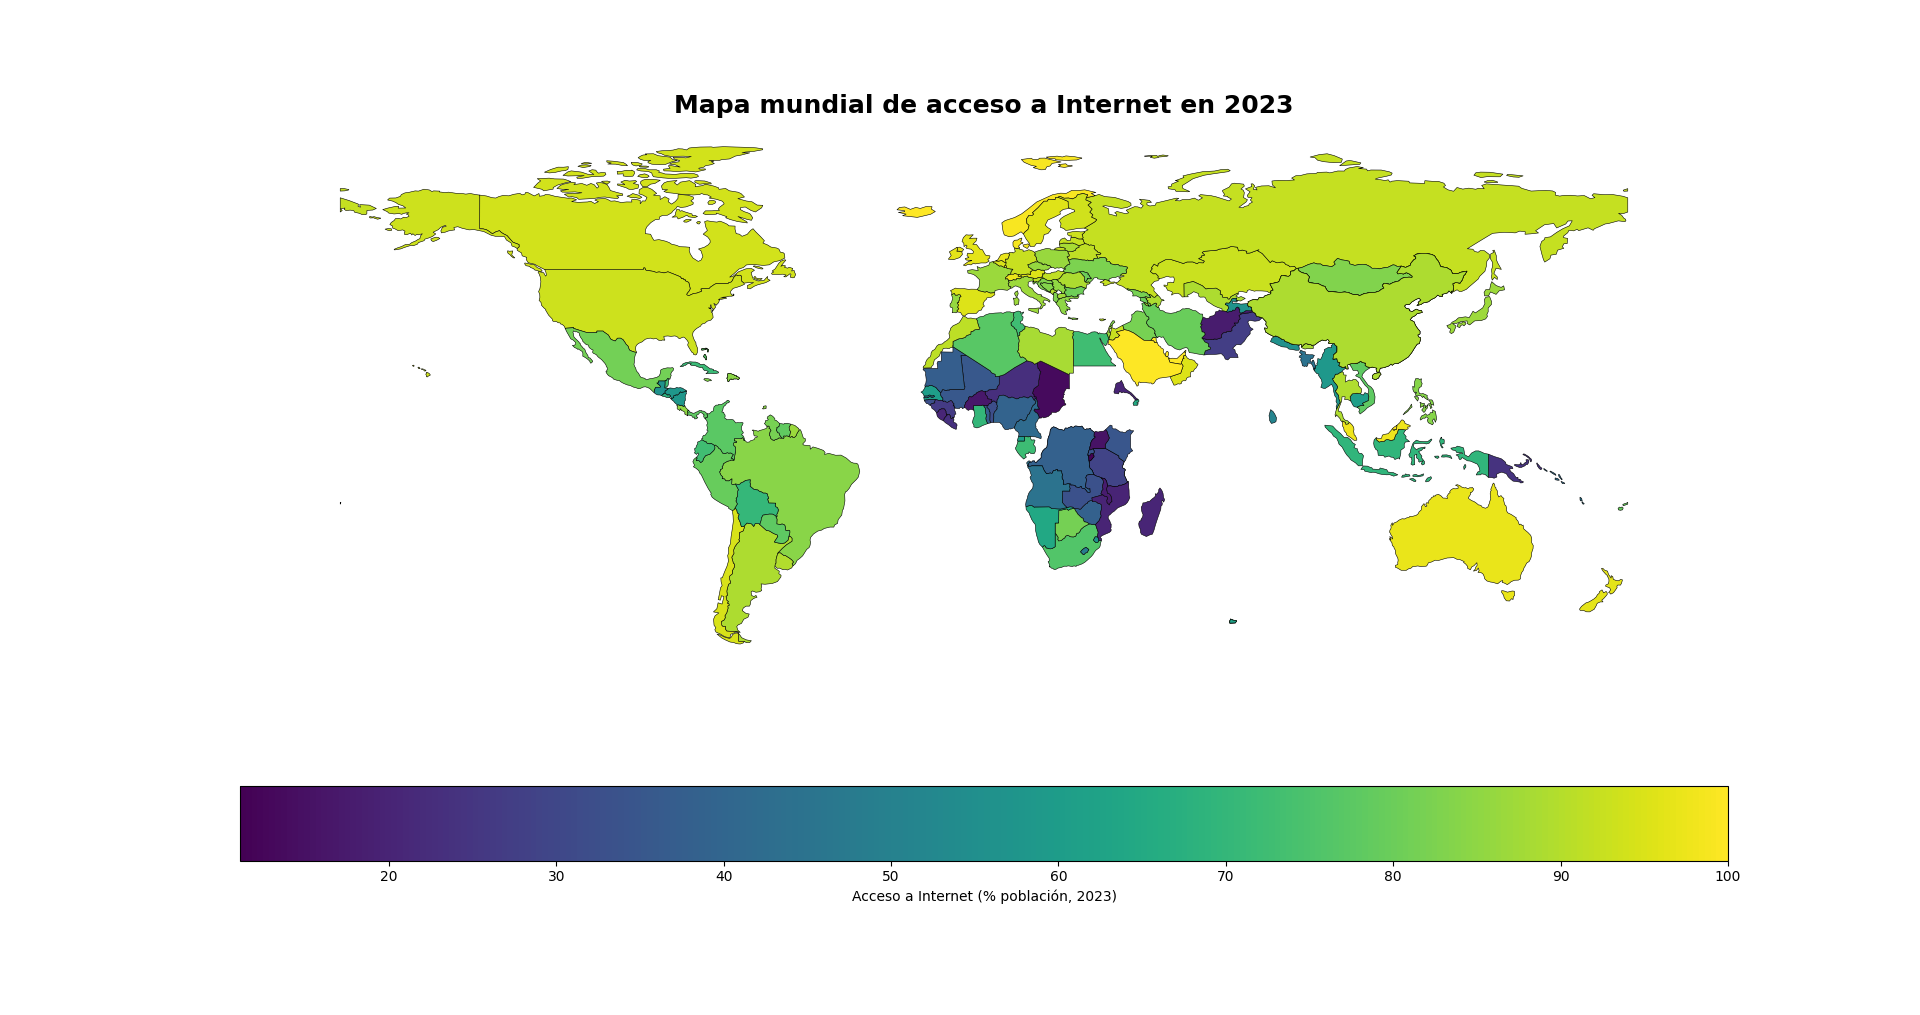
\includegraphics[width=0.85\textwidth]{Graficos/Grafico_uso_de_internet_FC.png}
    \caption[5]{Fuente: Elaboración propia con datos}
\end{figure}

\textbf{Conclusión:}  
\begin{itemize}
    \item Se puede observar una preocupación alta en todos los grupos presentando una mediana cercana a 4 a través de todos los rangos etarios.
    \item Al observar detalladamente cada violín se puede notar que los dos últimos rangos etarios (36-45 y 46+) poseen un valor mínimo de 1, lo que implica que existen encuestados pertenecientes a esos grupos que demuestran la preocupación mínima de 1 respecto al uso de sus datos personales, este no es el caso para los grupos más jóvenes (18-25 y 26-35) donde se observa que incluso los encuestados con menor preocupación poseen por lo menos un nivel ligero de esta.
    \item Junto con esto si nos centramos en los dos últimos grupos etarios, observando cada área, podemos ver que el grupo con edades de 36-45 años son el grupo con la menor preocupación, mostrando también la menor media indicada por la tercera línea horizontal.
\end{itemize}

\subsubsection*{Gráfico 4: Penetracion 5G por país.}
\begin{figure}[H]
    \centering
    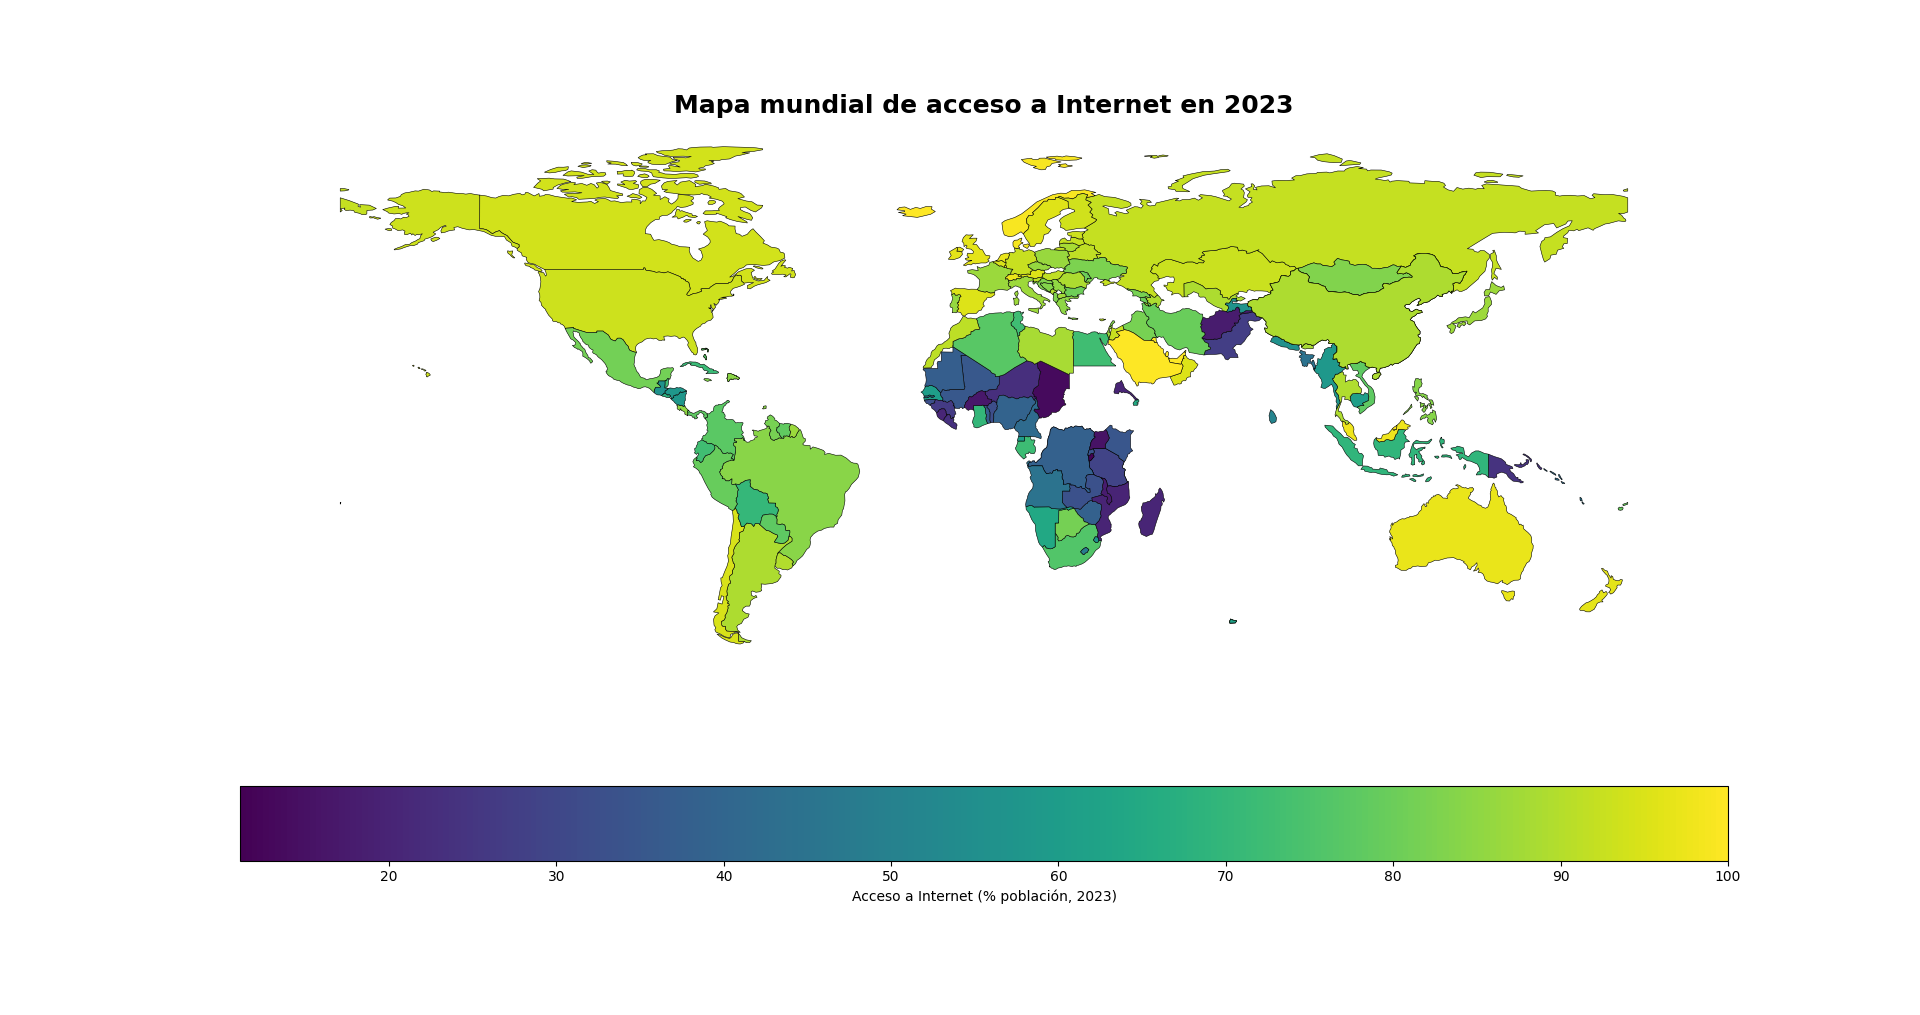
\includegraphics[width=0.85\textwidth]{Graficos/Grafico_uso_de_internet_FC.png}
    \caption[6]{Fuente: Elaboración propia con datos}

\end{figure}


\textbf{Conclusión:}  
\begin{itemize}
    \item Se observa que las curvas suben y bajan visiblemente para casi todos los países, en lugar de crecer de forma sostenida. Esto indica que la penetración 5G ha tenido retrocesos interanuales, lo cual puede deberse a factores técnicos, económicos o políticos que afectan el mantenimiento o la expansión de la red.
    \item Visualmente, países como Francia, Alemania y Japón presentan curvas más suaves y planas, lo cual sugiere un despliegue más progresivo y controlado en comparación con otros países donde hay caídas mas bruscas.

\end{itemize}

% ---------------------------------------------------------------------------------}
\section{Evidencia de encuesta aplicada}

A continuación, se presenta una imagen del archivo en Excel que contiene las respuestas recolectadas de la encuesta sobre el uso de inteligencia artificial. Esta tabla incluye los datos utilizados para generar los gráficos presentados anteriormente. Se realizo en google forms para mayor comodidad y cantidad de respuestas. 

\begin{figure}[H]
    \centering
    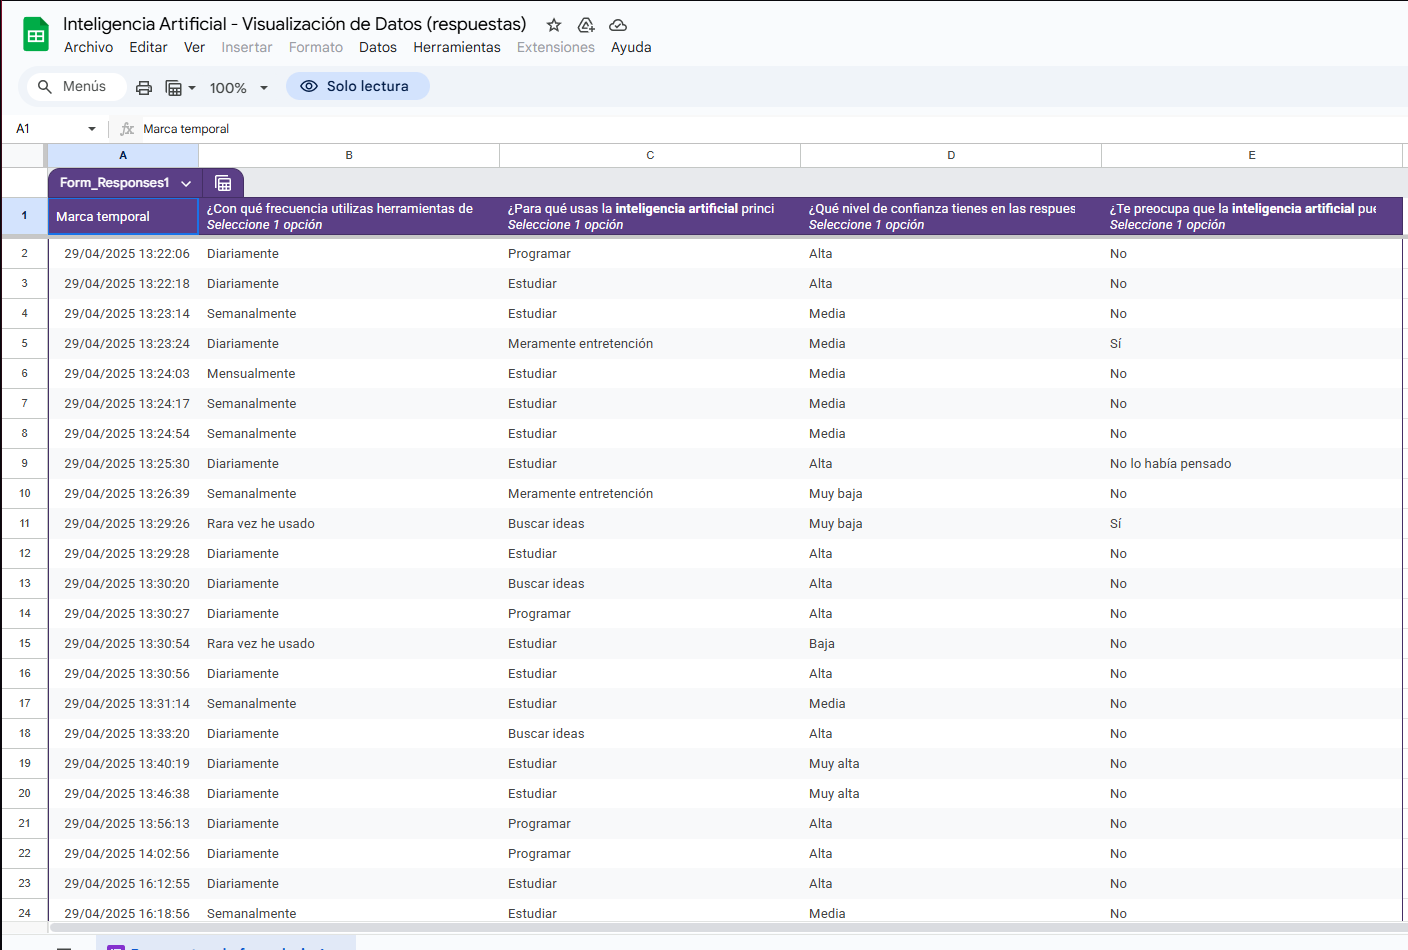
\includegraphics[width=0.95\textwidth]{Graficos/excel.png} % <-- nombre del archivo imagen
    \caption{Captura de pantalla del archivo Excel con las respuestas de la encuesta}
\end{figure}

El archivo completo puede ser consultado en el siguiente enlace:

\begin{itemize}
    \item \href{https://docs.google.com/spreadsheets/d/1KRdGL7pflDiA8TAT_pvPSt6OpXGPv6h4NTGceC8xDS0/edit?resourcekey=&gid=168064728#gid=168064728}{Ver archivo Excel de la encuesta}
\end{itemize}


\textbf{Repositorio:}  
\label{anexo:repositorio}

Acceso al repositorio en el siguiente link: 
\url{https://github.com/soloimsad/VD.git}

\end{document}
